\subsection{Syntax-number units interactions}[t]
\begin{figure*}
\centering
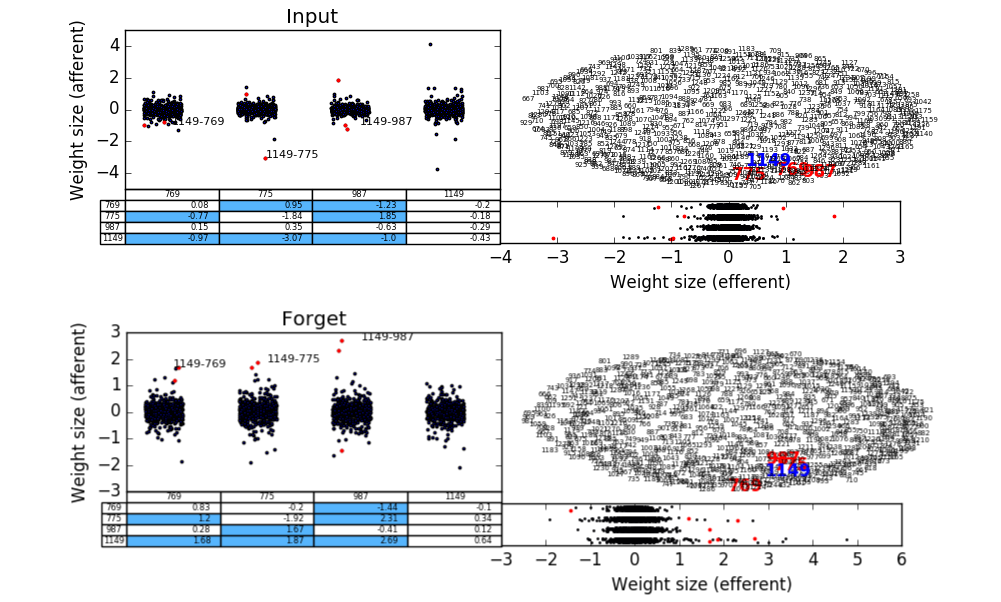
\includegraphics[width=\textwidth]{Figures/Figure7_interactions.png}
\caption{Interaction among the syntax and number units. A value in the table represents the weight size from the unit appearing on the left to the unit appearing on the top row. (A) Distribution of all weight values to the unit appearing on the top row of the table. Outlier weights from the table (more than three standard-deviation above/below the mean) are marked in red; Weight values from the syntax to number units have in addition a corresponding text label. (B) Distribution of all weight values from the unit appearing on the left column of the table. Outlier weights are marked in red. (C)  A visualization of unit interactions. For each gate $g$, an interaction distance $d_{ij}^g$ between a pair of units $i$ and $j$ was first defined as: $d_{ij}^g=exp{-max{w_{ij}^g, w_{ji}^g}}$, where $w_{ij}^g$ is the weight from unit $j$ to the gate $g$ of unit $i$. Then, all interaction distances in the network were visualized using multidimensional scaling. Note that the interaction distances between the number units and between the syntax and number units are relatively close compared to the mean interaction distance in the network.}
\end{figure*}

To explore the interaction between the syntax and LR-number units, we now look into the connectivity of the network, with a focus on the connection weights among these units. Note that for each pair of units that are four types of connection corresponding to the four types of gates: suggestion, input, forget and output gates. Each type of weight can thus contribute to a different type of interaction, depending on the function of the gate. Figure X shows the distribution of all afferent (top-left) and efferent (bottom-right) recurrent weights of units 776, 988 and 1150, for both input and forget gates (panels A\&B), and the tables show all weight values among the three units. In addition, we visualized the interactions among all units in networks in the following way: for each type of gate $g$ and a pair of units $i$ and $j$, we defined an interaction distance as: $d_{ij}=e^{-\max{\{|W_{ji}^{g}|, |W_{ij}^{g}|\}}}$. That is, the stronger the interaction between unit $i$ and $j$ is the closer these units are. The maximal possible distance is one, which corresponds to zero weights in both direction. Next, to visualize network interacitons, we projected all pairwise distances on the plane, using multi-dimensional scaling (MDS) (cite) (upper-right side of panels A\&B.).

From the MDS results, it is apparent that the interaction distances between the syntax and LR-number units are relatively small compared to the average distance in the network. This corresponds to both types of weights from the syntax unit 1150 to the LR-number units, which are exceptionally high compared to all afferent connections to the forget gates of the number units (rank, $p-value=$,), and exceptiaonlly low to their input gates (rank, $p-value$). This means that when the activity of the syntax unit is relatively high $h_1150 > 0$ the syntax unit is driving the forget gate of the number units towards a value of one (since, $W^f_{776, 1150}h_1150>0$) and their input gates towards a value of zero ($W^i_{776, 1150}h_1150<0$). Looking at the r.h.s. of equation X.X, this means that the first term becomes dominante and the second term goes to zero, meaning that in this way the syntax unit conveys a \textit{'remembering signal'} to the LR-number units, that is, to ignore any coming input and to keep the (number) information stored in the cell. similarly, when $h_1150<0$, the syntax unit conveys an 'updating signal' to the LR-number units, that is, to forget the stored number information in the cell and to refresh it with the new cell-suggestion value. Indeed, as shown in section 5.2, $h_1150$ is positive during the embedded phrase within the subject-verb dependency, which then changes abruptly to a negative value at the time point of the main verb. This is in accordance with the interpretation that the syntax unit 1150 controls the storage and update of grammatical-number information in the LR-number units - throughout the processing of the embedded phrase within the subject-verb dependency the syntax unit propagtes a 'remembering signal' to the LR-number units, and only when the main verb appears it signals to these units that it is time to forget the stored number infromation and update it. 

We also note that the weight values between the two LR-number units are significanly high compared to all other afferent connections. Given that their output activity $h_776$ and $h_988$ is negative during the storage of number information (Figure 2), this means that these units are \textit{mutually inhibiting}. In other words, when the singular unit stores the information that the subject is currently singular it inhibits the activity of the plural unit, and vice versa in the case of a plural subject. This seems to warrant an unequivocal signal about the grammatical number of the subject to the output layer.

\textcolor{red}{(perhaps for the discussion:) Interestingly, this meaningful 'neuroanatomy' and the intricate dynamics of the syntax and LR-number units have all emerged from the unlabelled language-model task of predicting the next work.}


